\subsubsection{Comunidades}
Actualmente el número de organizaciones que buscan compartir información de
amenazas es creciente. Esto lleva a que el número y tipo de comunidades que busca
hacerlo también se incremente. En la actualidad se identifican tres tipos de comunidades:
\begin{itemize}
  \item Pares
  \item Comerciales
  \item Gubernamentales
\end{itemize}

Para que se pueda compartir información entre dichas organizaciones es necesario
cierto nivel de confianza dado que compartir información sensible podría exponer 
a las organizaciones a daños en su reputación, demandas o advertir a un 
atacante de la investigación que se lleva a cabo haciendo que el trabajo 
realizado haya sido inútil. Se deben definir medidas para la protección de los 
datos como restricciones en su manejo, sanitización y el establecimiento de 
confianza entre las dos organizaciones. Lo mencionado anteriormente es 
particularmente importante cuando las organizaciones forman parte de varias 
comunidades que intercambian información, se encuentran casos en los que datos 
compartidos con una organización no deberían ser compartidos con otra.\\

Las comunidades entre \textbf{pares} son las más comunes, estas organizaciones o 
individuos tienen el propósito común de mejorar las defensas colectivas contra 
adversarios que tienen en común. La información compartida por dichas 
organizaciones es más especifica que la provista por organizaciones comerciales.\\

Las comunidades \textbf{comerciales} son anónimas y los miembros poseen algún tipo de 
acuerdo común, por ejemplo el pago de cuotas para pertenecer a la comunidad. 
La organización comercial maneja la información de forma centralizada y la 
distribuye entre los miembros de la organización. El acceso a la información por 
parte de los socios es rápido teniendo la posibilidad de que dicha información 
sea más amplia que la compartida por pares y que además no siempre sea aplicable a las 
necesidades de la organización.\\

Las comunidades \textbf{gubernamentales} son establecidas y manejadas por el gobierno, 
son voluntarias u obligatorias e incluyen participantes tanto del gobierno como 
de la industria privada. En ellas el gobierno controla la información y la 
distribución de esta. Así como en las comunidades comerciales, la información y 
los participantes son altamente confidenciales.\\

\subsubsection{Modelos}

Se pueden identificar tres modelos para el intercambio de información entre 
organizaciones:
\begin{itemize}
  \item Hub and Spoke
  \item Peer to peer
  \item Source/subscriber
\end{itemize}

En el método \textbf{hub and spoke}, la entidad hub controla la recepción y diseminación 
de los datos, además se encarga de mantener anónimos y proveer un análisis 
adicional de los datos recolectados para luego diseminarlos entre los 
participantes. Este modelo es comúnmente visto en comunidades de gobierno o comerciales.\\

En el modelo \textbf{peer to peer}, los participantes intercambian y reciben información 
directamente de los otros participantes. La información es compartida entre 
todos los miembros de la comunidad por igual y la fuente está claramente 
identificada.\\

\textbf{Source/subscriber} es utilizado por las 
comunidades comerciales que proveen de información. El proveedor de información 
envía regularmente información a todos los subscriptores y estos podrían 
eventualmente enviarle información a la fuente. Generalmente, la información se 
codifica de una manera propietaria y puede faltar información esencial sobre 
algunos intentos de irrupción. Presenta la ventaja de que se tiene acceso rápido 
a un conjunto de datos amplio y es útil para organizaciones con recursos 
limitados.\\

\subsubsection{Implementación de Modelos en TAXII}

A continuación se muestra como los servicios TAXII pueden ser utilizados para la 
implementación de los modelos para el intercambio de información.

\paragraph{Source/Suscriber}\ \\

En este modelo una entidad es la fuente de información y algunos subscriptores 
tienen acuerdos con dicha entidad para recibir información periódicamente. Se 
busca que los subscriptores no se conozcan entre si, para ello la entidad fuente 
realiza acuerdos con cada uno de ellos. En este modelo, la fuente es 
un productor TAXII mientras que los subscriptores son consumidores.\\

TAXII soporta este tipo de modelo para el intercambio con el uso de los servicios de 
Discovery, Feed Management, Inbox y Poll. Una organización que desee 
subscribirse al TAXII Data Feed de la fuente necesita conocer los servicios 
TAXII que la fuente ofrece y como contactar con ellos. Si bien esto podría ser 
realizado por una mecanismo fuera de banda (e.g. publicando la información en otro medio)
también podría ser logrado contactando al Discovery Service de la fuente. Desde 
este punto, el subscriptor podría contactar al servicio de Feed Managment 
identificado para aprender que fuentes ofrece el productor y que restricciones 
podría tener su acceso.\\

Si el contenido del TAXII Data Feed es restringido solo a algunas entidades 
autorizadas y el productor ha determinado que el subscriptor tiene permitido 
recibir el contenido, la fuente y el subscriptor necesitan acordar en como el 
subscriptor se autenticará. Dependiendo en el protocolo que soporta la fuente, 
esto se puede realizar por medio de una contraseña, un certificado u otro método. 
Si el contenido de un TAXII Data Feed es abierto y no requiere 
autenticación, éste paso es innecesario cuando se establecen las subscripciones 
al TAXII Data Feed.\\

Luego de la autenticación,el subscriptor puede contactar al Feed Managment Service del 
productor y pedir subscripciones a sus fuentes. La entidad fuente puede 
comparar dichos pedidos con su propio entendimiento de lo que el subscriptor 
puede recibir y permitir o denegar dichos pedidos según corresponda. La fuente 
puede enviar contenido al subscriptor al Inbox Service de éste en el intervalo 
apropiado. Alternativamente, el subscriptor podría contactar al Poll service de 
la fuente para descargar el contenido deseado.\\

\begin{figure}[ht!]
 
  \centering
  	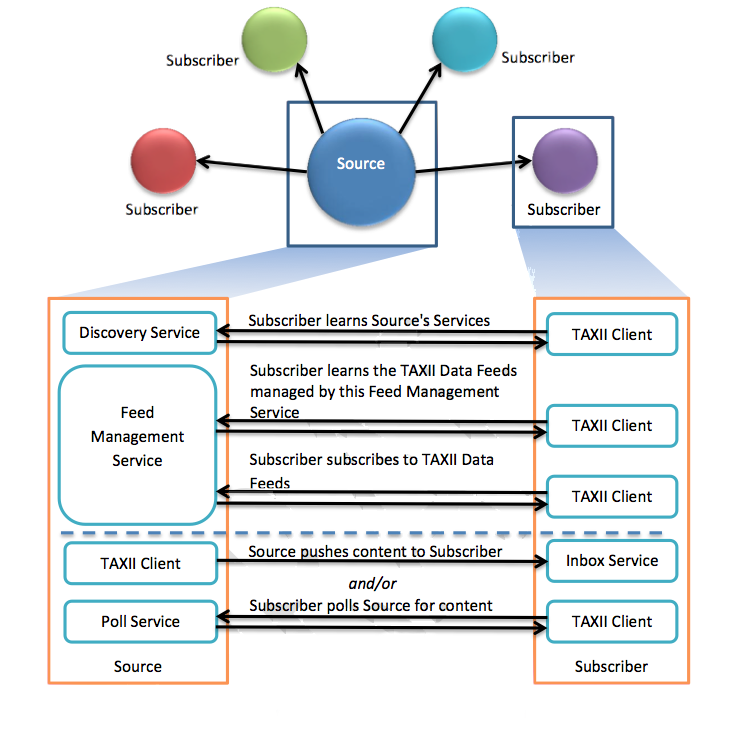
\includegraphics[width=150mm]{./images/SourceSuscriberModel.png}
    \caption{Flujo de información en modelo Source/Subscriber \protect\cite{b1}}
    \label{fig.sourcesuscribermodel}
\end{figure}

La figura \ref{fig.sourcesuscribermodel} muestra como el modelo Source/Subscriber puede ser soportado por los 
servicios TAXII. También se ven los mensajes TAXII intercambiados entre la
fuente y el subscriptor. Con los intercambios que están por encima de la línea 
punteada se establece la subscripción. Los intercambios pueden ser realizados 
repetidamente sin la necesidad de realizar el proceso de subscripción 
nuevamente.

\newpage

\paragraph{Peer-to-peer}\ \\ 

En un modelo Peer-to-peer, los pares de organizaciones entran en un acuerdo 
mutuo para compartir información entre si. En este modelo, cada Peer puede 
operar como productor y consumidor. Los socios en este intercambio podrían 
establecer fuentes utilizando un procedimiento similar al establecido en el 
modelo Source/Subscriber. Alternativamente, podrían acordar subir o descargar 
contenido sin ninguna subscripción formal. No tener una subscripción formal 
permite a un Peer albergar un Inbox Service sin necesidad de un Feed 
Managment Service.\\

El modelo Peer-to-Peer tiene dos variantes: acuerdos para el intercambio entre 
comunidades y acuerdos para el intercambio ad-hoc. En el primero la comunidad 
constituye acuerdos entre pares en los que todos los miembros acuerdan una única 
política la cual será respetada por todos. A diferencia de los otros dos 
modelos que tienen un punto central desde el cual la información es diseminada, 
todo el intercambio ocurre puntualmente entre dos pares. Si los pares A y B 
desean recibir información del peer C directamente, ambos necesitaran 
establecer un acuerdo apropiado con el peer C para que éste les envíe la 
información que desean.\\

Alternativamente, el intercambio entre pares puede ser realizado de forma 
individual con intercambios ad-hoc. Esto podría ocurrir si dos compañías hacen 
acuerdos individuales para compartir entre ellas. En este caso, los acuerdos 
sobre que compartir son específicos para las partes. Una sola entidad podría 
participar en ambas variantes, perteneciendo a una o mas comunidades en las 
cuales los miembros comparten entre si siguiendo un acuerdo común entre los 
miembros y a su vez negocian acuerdos individuales con otras entidades. Alguna 
información recibida por medio de un acuerdo no siempre debería ser compartida 
con otros pares que no son parte del acuerdo. De esta forma un participante 
debería hacer un seguimiento de quien fue el proveedor de la información 
recibida, como se realiza ese seguimiento está por fuera de la especificación de 
TAXII.\\

\begin{figure}[ht!]
  \centering
  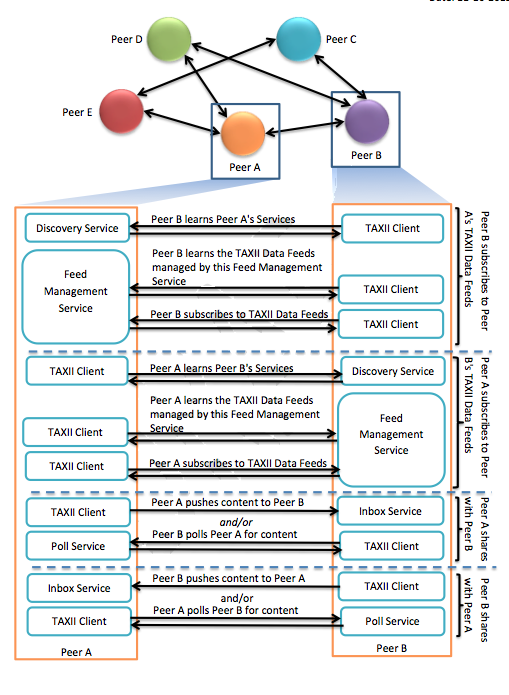
\includegraphics[scale=0.55]{./images/PeerToPeerModel.png}
    \caption{Flujo de información en modelo Peer to Peer \protect\cite{b1}}
  \label{fig.peertopeermodel}
\end{figure}

La figura \ref{fig.peertopeermodel} muestra como el modelo Peer to peer puede ser realizado por 
medio de los servicios TAXII. En este diagrama se ve que dos pares se contactan 
para pedir subscripciones para obtener información. Se asume que ambos pares 
tienen un Feed Managment Service que es utilizado para manejar todos los 
pedidos de subscripción.
\newpage

\paragraph{Hub and Spoke}\ \\

En un modelo Hub and Spoke, la entidad Hub es un consumidor de 
información, dicha información es provista por las entidades Spoke, pero a su vez se comporta como
un productor que brinda información a entidades 
Spoke. Una entidad Spoke podría ser un productor, dando información al Hub, un 
consumidor que reciba actualizaciones del Hub o ambas. El Hub puede utilizar un 
Inbox Service para recibir información de cualquiera que desee enviar 
información de forma voluntaria y/o podría requerir información de ciertas 
fuentes para guardar la información en una única ubicación. Desde este punto, el 
Hub puede funcionar como una entidad Source del modelo Source/Subscriber 
mientras que los Spoke serían Subscribers de dicho modelo. El Hub puede adoptar 
cualquier política respecto de la información que recibe, desde pasar toda la 
información automáticamente a solo pasar información de socios reconocidos, o 
realizar ediciones y análisis antes de reenviar la información.

\begin{figure}[ht!]
  \centering
    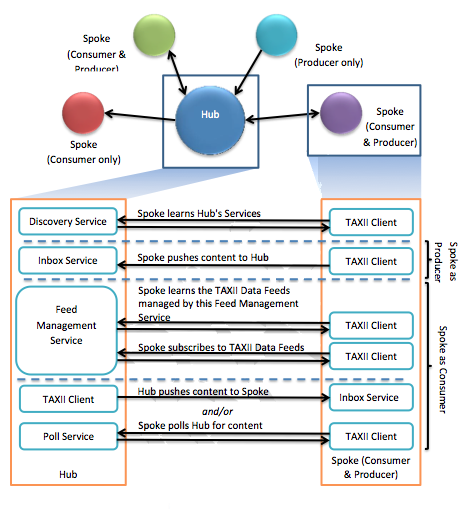
\includegraphics[scale=0.75]{./images/HubAndSpokeModel.png}
    \caption{Flujo de información en modelo Hub and Spoke \protect\cite{b1}}
    \label{fig.hubandspokemodel}
\end{figure}

La figura \ref{fig.hubandspokemodel} muestra como se puede implementar el modelo Hub and Spoke 
utilizando los servicios provistos por TAXII. En este modelo algunas entidades 
Spoke podrían ser consumidores, otras productores y en algunos casos ambas. El 
diagrama muestra los intercambios que podrían ser utilizados por el Spoke que 
actúa como productor y consumidor. Si este desea actuar de una sola forma solo 
los intercambios necesarios serían relevantes. Independientemente del rol que 
tome el Spoke, es necesario que éste conozca los servicios relevantes en el Hub. 
Esto se realiza utilizando el Discovery Service provisto por el Hub, de todas 
formas esto podría realizarse con mecanismos fuera de banda.



